%iffalse
\let\negmedspace\undefined
\let\negthickspace\undefined
\documentclass[journal,12pt,twocolumn]{IEEEtran}
\usepackage{cite}
\usepackage{amsmath,amssymb,amsfonts,amsthm}
\usepackage{algorithmic}
\usepackage{graphicx}
\usepackage{textcomp}
\usepackage{xcolor}
\usepackage{txfonts}
\usepackage{listings}
\usepackage{enumitem}
\usepackage{mathtools}
\usepackage{gensymb}
\usepackage{comment}
\usepackage[breaklinks=true]{hyperref}
\usepackage{tkz-euclide} 
\usepackage{listings}
\usepackage{gvv}                                        
%\def\inputGnumericTable{}                                 
\usepackage[latin1]{inputenc}                                
\usepackage{color}                                            
\usepackage{array}                                            
\usepackage{longtable}                                       
\usepackage{calc}                                             
\usepackage{multirow}                                         
\usepackage{hhline}                                           
\usepackage{ifthen}                                           
\usepackage{lscape}
\usepackage{tabularx}
\usepackage{array}
\usepackage{float}
\usepackage{circuitikz}


\newtheorem{theorem}{Theorem}[section]
\newtheorem{problem}{Problem}
\newtheorem{proposition}{Proposition}[section]
\newtheorem{lemma}{Lemma}[section]
\newtheorem{corollary}[theorem]{Corollary}
\newtheorem{example}{Example}[section]
\newtheorem{definition}[problem]{Definition}
\newcommand{\BEQA}{\begin{eqnarray}}
\newcommand{\EEQA}{\end{eqnarray}}
\newcommand{\define}{\stackrel{\triangle}{=}}
\theoremstyle{remark}
\newtheorem{rem}{Remark}

% Marks the beginning of the document
\begin{document}
\bibliographystyle{IEEEtran}
\vspace{3cm}

\title{Electric Circuit}
\author{AI24BTECH11015 - Harshvardhan Patidar}
\maketitle
\newpage
\bigskip

\renewcommand{\thefigure}{\theenumi}
\renewcommand{\thetable}{\theenumi}


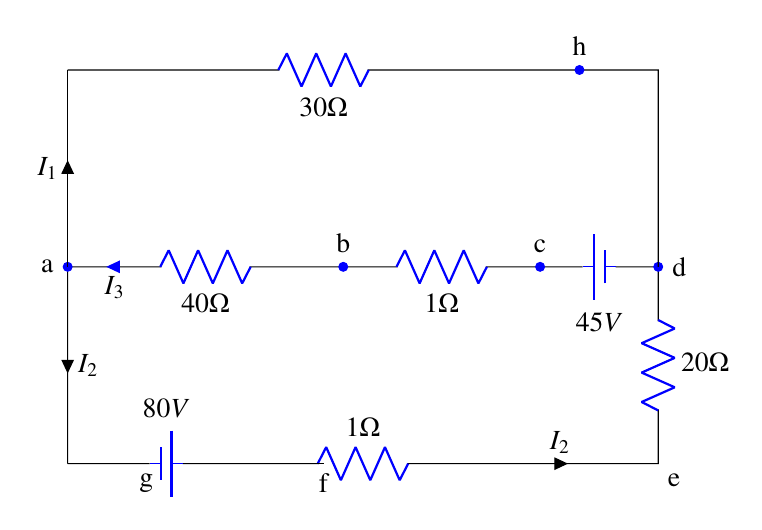
\begin{tikzpicture}
        %Drawing the lower loop
        \draw   (0,0) to[battery1, invert, color=blue, l=$80V$, ]
                (2.5,0) to[R, l=$1 \ohm$, color=blue,]
                (5,0) to[short, i=$I_2$]
                (7.5,0) node[anchor=north west] {e} to[R, l_=$20\ohm$, color=blue] 
                (7.5,2.5) node[circ, color=blue, label=east:d]{} to[battery1, l=$45V$, color=blue, invert] 
                (6,2.5) node[circ, color=blue, label=north:c]{} to[R, color=blue, l=$1\ohm$] 
                (3.5,2.5) node[circ, color=blue, label=north:b] {} to[R, color=blue, l=$40\ohm$, i>=$I_3$] 
                (0,2.5) node[circ, color=blue, label=west:a]{} to[short, i=$I_2$]
                (0,0);
        %drawing the wire from d to h and the horizontal wire only
        \draw   (7.5,2.5) to 
                (7.5,5) to 
                (6.5,5) node[circ, color=blue, label=north:h]{} to[R, color=blue, l=$30\ohm$]
                (0,5);
        %drawing the vertical i1 vala wire
        \draw   (0,2.5) to[short, i=$I_1$]
                (0,5);             

        %Putting in the label g by a jugaad
        \draw   (1,0) node[anchor=north]{g} to
                (0,0);

        %doing the same for f
        \draw   (3.25,0) node[anchor=north]{f} to
                (3,0);
        \end{tikzpicture}
\end{document}
